\section{Vorgehen in Regelungstechnik}
Zur Ermöglichung einer strukturierten Vorgehensweise bedarf es einer Orientierung. Dieser Arbeit liegt die in der Vorlesung behandelte Vorgehensweise in der Regelungstechnik zugrunde, welche nachfolgend erläutert wird.

\begin{enumerate}
    \item Detaillierungsgrad für das System festlegen
    \item Physikalisches Modell einschließlich der Störsignale erstellen
    \item Eingangs-, Ausgangs-, Zustands- und Störgrößen des Systems festlegen
    \label{Punkt3}
    \item Physikalische Einheiten festlegen und ggf. Normierung in Prozent
    \label{Punkt4}
    \item Analyse des Modells
    \label{Punkt5}
    \begin{enumerate}
        \item Ruhelagen, Anfangswerte, evtl. Linearisierung nichtlinearer Systeme
        \item Systemeigenschaften ermitteln
    \end{enumerate}
    \item Entwurf
    \label{Punkt6}
    \begin{enumerate}
        \item Ziele, Arbeitspunkte und Trajektorien festlegen
        \item Entwurf: Struktur, Bereich, Verfahren und Kriterien
    \end{enumerate}
    \item Simulation und Rückinterpretation
    \label{Punkt7}
\end{enumerate}

In dieser Vorlesung wird die Regelungstechnik außen vor gelassen, weswegen im Folgenden eine leicht abgewandelte Struktur angewendet wird. Bezüglich des Detaillierungsgrads sind alle in der Vorlesung behandelten Darstellungsformen darzulegen. Weiterführend werden die Punkte \hyperref[Punkt3]{3} und \hyperref[Punkt4]{4} des Vorgehens aus der Regelungstechnik zusammengefasst und tabellarisch dargestellt. Schwerpunktmäßig wird in dieser Arbeit Punkt \hyperref[Punkt5]{5} behandelt, in dem alle Darstellungsformen aus der Vorlesung dargelegt werden. Punkt \hyperref[Punkt6]{6} und \hyperref[Punkt7]{7} werden in dieser Arbeit nicht betrachtet.

\section{Unser System}
Wir betrachten einen Wassertank, der oben an einen Zufluss mit sehr hohem Druck angeschlossen ist. Am unten Ende des Wassertanks befindet sich ein deutlich kleinerer Abfluss, an den eine lange Wasserleitung angeschlossen ist. Erst am Ende der Wasserleitung befindet sich ein Messgerät, welcher den Volumenstrom misst.
Eine beispielhafte Skizze sieht folgendermaßen aus:
\begin{figure}[H]
    \label{fig:tank}
    \centering
    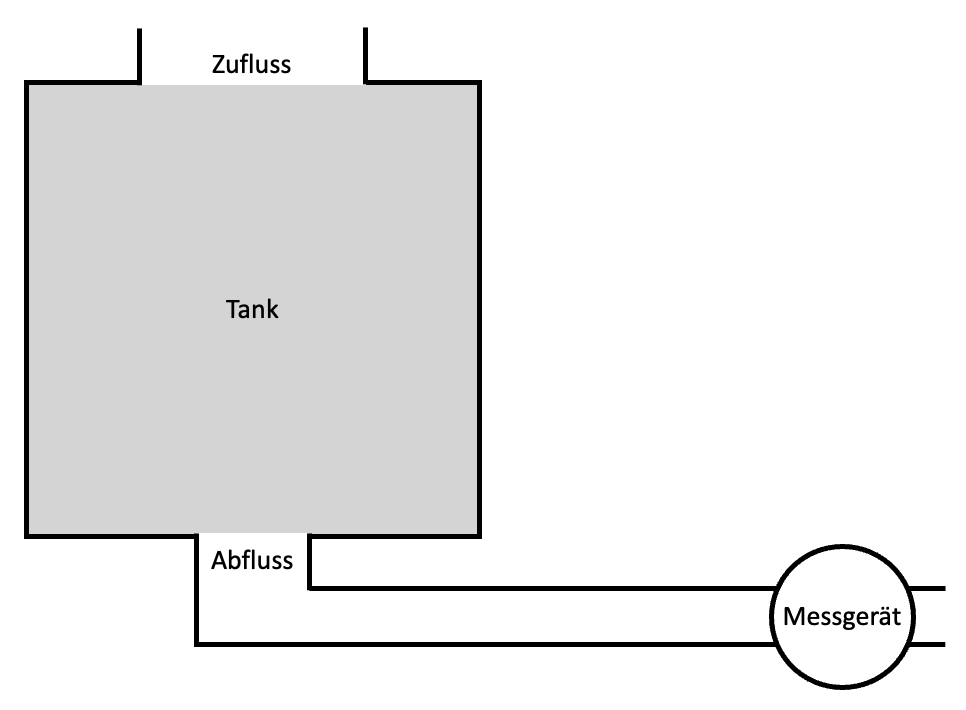
\includegraphics[width=0.8\textwidth]{Bilder/Tank.png}
    \caption{Skizze des Systems}
 \end{figure}
Der Ablauf stellt sich wie folgt dar: Über den Zufluss fließt Wasser in den Tank. Da der Abfluss aber deutlich kleiner ist, fließt erstmal deutlich weniger Wasser heraus. Erst wenn der Tank voller wird, erhöht sich der Druck und es kommt zu einem immer größeren Volumenstrom bis der Tank schließlich so voll (Wasser und komprimierte Luft) ist, dass der Druck des Zuflusses dafür sorgt, dass der Volumenstrom am Abfluss gleich dem am Zufluss ist. Da das Messgerät aber weit entfernt vom Tank liegt, misst dieses den ganzen Vorgang erst mit einer gewissen Verzögerung.

Je nachdem wie groß der Tank ist, verändert sich die Konstante $T_1$: Je kleiner der Tank, desto größer ist $T_1$. Aber auch das Verhältnis von Zuflussgröße zu Abflussgrößte beinflusst die Konstante $T_1$. Gleichzeitig bestimmt der Abstand zwischen dem Tank und dem Messgerät die Zeitkonstante $T_t$: Je größer der Abstand, destor größer ist $T_t$.

\subsection{Größen}
Im Folgenden werden Eingangs-, Zustands- und Ausgangsgrößen des Systems definiert.
\renewcommand{\arraystretch}{1.5}
\begin{center}
    \begin{tabular}{ c|c|l } 
    Systemtheorie  & Größe im System & Einheit \\
    \hline
    $u(t)$ & Volumenstrom am Zufluss & $\frac{l}{min}$ \\ 
    $x(t)$ & Volumenstrom am Abfluss &  $\frac{l}{min}$\\ 
    $y(t)$ & Volumenstrom am Messgerät & $\frac{l}{min}$ \\ 
    \end{tabular}
\end{center}
%Die Eingangsgröße $u(t)$ ist in unserem Beispiel der Volumenstrom am Zufluss, angegeben z.\,B. in $\frac{l}{min}$. Der Zustand $x(t)$ ist der Volumenstrom am Abfluss und der Ausgang $y(t)$ ist der gemessene Volumenstrom am Messgerät.


\subsection{Bezeichnung}
Das System hat den Nennergrad 1, eine Totzeit $T_t$ und ein proportionales Übertragungsverhalten. Daraus ergibt sich die Bezeichnung $PT_{1}T_{t}$.

\subsection{Übertragungsfunktion}

Formel \ref{eq:G(s)_1} zeigt die Übertragungsfunktion die in diesem Skript analysiert wird. Dabei gehen wir bei unserem System gehen davon aus, dass $T_1$ gleich 1 und $T_t$ gleich 2 ist. Formel \ref{eq:G(s)_3} zeigt eine etwas andere Darstellung der Formel, sodass die Eigenschaften des Systems leichter abzulesen sind.

\begin{eqnarray}
    \label{eq:G(s)_1}
    G(s) &=& \frac{Y(s)}{U(s)} \\
    \label{eq:G(s)_2}
    &=& \frac{1 \cdot e^{-2s}}{1+s} \\
    \label{eq:G(s)_3}
    &=& \frac{1}{1 + s} \cdot e^{-2s}
\end{eqnarray}

\subsection{Eingabe in Matlab}
Für die Eingabe der Übertragungsfunktion in Matlab gibt es zwei Möglichkeiten. \\
In Computer-Algebra führt man \texttt{s} und \texttt{G(s)} als symbolischen Variablen ein und kann anschließend die Übertragungsfunktion \texttt{G(s)} definieren:

\begin{verbatim}
    syms s, G(s)
    G(s) =  1 / (1 + s) \cdot exp(-2 \cdot s)
\end{verbatim}

Man erhält dasselbe Ergebnis wie bei der obigen manuellen Definition von $s$ und $G(s)$, wenn man den Transfer-Function-Befehl \texttt{tf()} in Matlab verwendet:

\begin{verbatim}
    sys = tf([1], [1, 1],\textquotedbl IODelay\textquotedbl, 2)
\end{verbatim}

Hierbei werden in den beiden Vektoren die Koeffizienten vor $s^0$, $s^1$, $s^2$, \ldots im Zähler und im Nenner angegeben. Bei komplizierteren Gleichungen hilft dabei der Befehl \texttt{expand(G(s))}, der einem die benötigten Koeffizienten liefert, was hier jedoch nicht nötig war. Darauf folgt der Befehl \texttt{\textquotedbl IODelay\textquotedbl}, mit dem die Totzeit $t = 2$ angegeben wird.

In beiden Fällen wird in Matlab damit die Formel \ref{eq:G(s)_3} dargestellt.

\section{Darstellungsformen des Systems}
Im Folgenden werden die Darstellungen unseres Systems näher beleuchtet. Generell gilt: Mit jeder weiteren Darstellung verliert man bestimmte Informationen über das System, sodass die erste Darstellung die informationsreichste ist.

\subsection{Explizite Darstellung des Übertragungsoperators}

\subsection{Zustandsraumdarstellung}
Der Zustandsraum lässt sich sowohl implizit als auch explizit darstellen.

\subsubsection{Implizite Darstellung}

Die allgemeine Form der Zustandsraumdarstellung lautet:
\begin{align*}
    \dot x & = Ax + Bu \nonumber \\
    y & = Cx + Du
\end{align*}

Mit dem Matlab-Befehl \texttt{ss(sys)} (ss steht für State Space) berechnet Matlab automatisch die Werte für unser System. Somit ergibt sich für unser System die folgende Zustandsraumdarstellung:
\begin{align*}
    \dot x & = \begin{bmatrix}
        -1
    \end{bmatrix}x + \begin{bmatrix}
        1
    \end{bmatrix}u \\
    y & = \begin{bmatrix}
        1
    \end{bmatrix}x + \begin{bmatrix}
        0
    \end{bmatrix}u
\end{align*}

Sind die Matrizen $A, B, C, D$ eines Systems bekannt, kommt man mit der folgenden Formel zur Übertragungsfunktion $G(s)$, wobei $I$ die Einheitsmatrix darstellt.
\[
    G(s) = C(s \cdot I - A)^{-1} \cdot B + D
\]

Sofern die Matrizen gegeben sind, könnte man das System alternativ auch mit der dazugehörigen Zustandsraumdarstellung übergeben, indem \texttt{sys = ss(A, B, C, D)} in Matlab eingegeben wird. Der Befehlt \texttt{tf(sys)} liefert dann die Übertragungsfunktion über die Zustandsraumdarstellung.

In unserem System erhält man damit aber nicht die eigentliche Übertragungsfunktion, da die Totzeit $T_t$ verloren geht.

Für die Funktionalbeziehung eines Totzeitglieds im Zeitbereich gilt: $y(t) = u(t-T_t)$. Somit ergibt sich für die Zustandsraumdarstellung eines zeitverzögerten Systems:
\begin{align*}
    \dot x(t) & = Ax(t) + Bu(t - T_t) \nonumber \\
    y(t) & = Cx(t) + Du(t - T_t)
\end{align*}
In unserem System mit $T_t = 2$ bedeutet das also:
\begin{align*}
    \dot x(t) & = \begin{bmatrix}
        -1
    \end{bmatrix}x(t) + \begin{bmatrix}
        1
    \end{bmatrix}u(t - 2) \nonumber \\
    y(t) & = \begin{bmatrix}
        1
    \end{bmatrix}x(t) + \begin{bmatrix}
        0
    \end{bmatrix}u(t - 2)
\end{align*}

--> HIER NOCHMAL GROELL NACHFRAGEN
Anhand der Matrix $D$, die in unserem nur eine Nullmatrix ist, lässt sich ablesen, dass es sich hier um ein nicht sprungfähiges System handelt.

Ohne Matlab kann die Zustandsraumdarstellung in einfachen Fällen mithilfe des Substitutionstricks aus der Übertragungsfunktion erstellt werden. Für Systeme, bei denen auch $\dot u, \ddot u, \ldots$ in der Differentialgleichung vorkommt, ist das Ganze ein bisschen komplizierter, wird aber in \href{https://de.wikipedia.org/wiki/Zustandsraumdarstellung#Regelungsnormalform}{Wikipedia} beschrieben und kann entsprechend angewendet werden. Bei sprungfähigen Systemen sieht das noch etwas anders aus und es muss erst eine Polynomdivision gemacht werden, um $D$ zu erhalten. Im Mehrgrößenfall ist es noch komplizierter.

\subsubsection*{Anfangswerte}

Für die Simulation sind Anfangswerte notwendig, da der Start der Funktion definiert sein muss. Hierbei müssen die linken Grenzwerte verwendet werden, da sonst eventuelle Sprünge miteinbezogen würden. Es gilt:
\begin{align*}
    y(0^-) & = Cx(0^-) + Du(0^-) \\
    \dot y(0^-) & = CAx(0^-) + CBu(0^-) + D \dot u (0^-)
\end{align*}

Die Summanden, in denen $\dot u, \ddot u, \ldots$ vorkommt, können vernachlässigt werden. Schließlich sind die linksseiten Anfangswerte aufgrund der Heavyside-Funktion gleich 0.
Darüber hinaus gibt es einen Zusammenhang mit der Ein-/Ausgangs-Differentialgleichung: Die Anfangswerte des Zustandsraumes $x$ müssen mit denen der Ein-/Ausgangs- Differentialgleichung $y$ korrespondieren. Zur Berechnung werden folgende Formeln verwendet:

\begin{align*}
    \left(\begin{array}{c} y \\ \dot y \\ \ddot y \end{array}\right) &= \left(\begin{array}{l} c^T \\ C^T A \\ C^T A^2 \end{array}\right) \left(\begin{array}{c} x_1 \\ x_2 \\ x_3 \end{array}\right) \\
    \left(\begin{array}{c} x_1 \\ x_2 \\ x_3 \end{array}\right) &= \left(\begin{array}{l} C^T \\ C^T A \\ C^T A^2 \end{array}\right)^{-1} \left(\begin{array}{c} y \\ \dot y \\ \ddot y \end{array}\right)
\end{align*}

Weiterhin gehen wir bei unserem System davon aus, dass der Tank zu Beginn leer ist, somit kein Abfluss vorliegt. Daraus ergibt sich $x(0^-) = 0$ und mit voriger Formel gilt:
\begin{align*}
    \left(\begin{array}{c} y \\ \dot y \end{array}\right) &= \left(\begin{array}{c}0\\0\end{array}\right) \\
    \left(\begin{array}{c} x_1 \\ x_2 \end{array}\right) &= \left(\begin{array}{c}0\\0\end{array}\right)
\end{align*}


\subsubsection{Explizite Darstellung}

Mit den Anfangswerten lässt sich $x(t)$ und $y(t)$ explizit berechnen:

\begin{align*}
    x(t) & = e^{A(t-t_0)} \cdot x(0) + \int_{0}^{t} e^{A(t-t_0)}Bu(\tau) \,d\tau \nonumber \\
    y(t) & = Ce^{A(t-t_0)} \cdot x(0) + C \int_{0}^{t} e^{A(t-t_0)}Bu(\tau) \,d\tau + Du(t)
\end{align*}

Hier ist bei der Eingabe in Matlab wichtig zu beachten, dass für $e^{(\ldots)}$ nicht \texttt{exp}, sondern \texttt{expm}, verwendet wird, da man hier die Matrizenmultiplikation benötigt.


\subsubsection{Integralgleichung}
Im Gegensatz zur Differentialgleichung ergibt die Integralgleichung \enquote{mild solutions}, welche Sprünge abbilden können.
Als Integralgleichung gilt:
\begin{align*}
    x(t) & = x(0) + \int_{0}^{t} Ax(\tau) + Bu(\tau)\,d\tau
\end{align*}
Für unser System ergibt sich somit:
\begin{align*}
    x(t) & = \int_{0}^{t} \begin{bmatrix}
        -1
    \end{bmatrix}x(\tau) + \begin{bmatrix}
        1
    \end{bmatrix}u(\tau)\,d\tau
\end{align*}

TODO: JONAS KOMMENTAR: WAS DAVON IST EXPLIZITE ZUSTANDSRAUMDARSTELLUNG UND WAS IST INTEGRALGLEICHUNG

\subsubsection{Differentialgleichung}
Aus unserem physikalischen Modells lässt sich folgende Differenzialgleichung ableiten:
\begin{align*}
    y(t) & = x(t - 2) \\
    u(t) & = \dot x + x \\
    \dot x & = u - x\\
    y(t) & = x(t - 2) \\
\end{align*}

--> HIER NOCHMAL GROELL NACHFRAGEN

\subsection{Ein- /Ausgangs Differentialgleichung}
Für unser System ergibt sich unter Vernachlässigung des Totzeitglieds:
\begin{align*}
    G(s) &= \frac{1}{1 + s} \cdot e^{-2s}\\
G_{PT_1}(s) =\frac{Y(s)}{U(s)} &= \frac{1}{1 + s} \\
Y(s)(1+s) &= (1) \cdot U(s) \\
Y(s) + Y(s) \cdot s &= 1\cdot U(s) \\
\dot y(t) + y(t) &= u(t) 
\end{align*}

In dieser Differentialgleichung taucht die Totzeit $T_t$ nicht auf, da das Totzeitglied nicht mit einer gewöhnlichen Differentialgleichung beschrieben werden kann. Für die Funktionalbeziehung eines Totzeitglieds im Zeitbereich gilt: $y(t) = u(t-T_t)$. Für unser System mit der Totzeit $T_t = 2$ folgt somit:
\begin{align*}
    \dot y(t) + y(t) &= u(t - 2) 
\end{align*}
--> HIER NOCHMAL GROELL NACHFRAGEN



\subsection{Übertragungsfunktion}

Formel \ref{eq:2G(s)_1} zeigt die Übertragungsfunktion die in diesem Skript analysiert wird. Dabei gehen wir bei unserem System gehen davon aus, dass $T_1$ gleich 1 und $T_t$ gleich 2 ist.Formel \ref{eq:2G(s)_3} zeigt eine etwas andere Darstellung der Formel, sodass die Eigenschaften des Systems leichter abzulesen sind.

\begin{eqnarray}
    \label{eq:2G(s)_1}
    G(s) &=& \frac{Y(s)}{U(s)} \\
    \label{eq:2G(s)_2}
    &=& \frac{1 \cdot e^{-2s}}{(1+s)} \\
    \label{eq:2G(s)_3}
    &=& \frac{1}{1 + s} \cdot e^{-2s}
\end{eqnarray}

\subsection{Systemantworten}
Im Folgenden werden die Antworten des Systems auf den Dirac-Impuls $\delta(t)$ und den Einheitssprung $\sigma (t)$ näher erläutert.
Die Sprungantwort $h(t)$ und die Impulsantwort $g(t)$ sind jeweils ineinander überführbar: Durch Differenzieren von $h(t)$ erhält man $g(t)$ und durch Integrieren von $g(t)$ erhält man $h(t)$.
\subsubsection{Gewichtsfunktion (Impulsantwort)}
TODO: JONAS KOMMENTAR: PASST DAS VON DER BENENNUNG?
Die Gewichtsfunktion $g(t)$ wird auch als Impulsantwort bezeichnet.
Die Impulsantwort ist die Antwort eines Sytems auf einen Dirac-Impuls $\delta(t)$.\\
In Matlab lässt sich die Gewichtsfunktion sowohl graphisch ausgeben als auch analytisch berechnen.
Mithilfe des Befehls \texttt{ilaplace()}, wird die laplace-Transformierte  Gewichtsfunktion $g(t)$ zurückliefert:
\begin{verbatim}
    syms g(t)
    g(t) = ilaplace(G(s))
\end{verbatim}

Matlab Ausgabe: \texttt{g(t) = heaviside(t - 2)*exp(2 - t)}\\
Mathematische Notation: 
\begin{align*}
    g(t) &=1(t-2)\cdot e^{(2-t)}
\end{align*} wobei $1(t)$ für die Heavyside-Funktion steht.

Mit dem Matlab-Befehl \texttt{impulse(sys)} wird ein Plot der Impulsantwort erstellt, was in folgender Abbildung zu sehen ist. 

\begin{figure}[H]
    \label{fig:impuls}
    \centering
    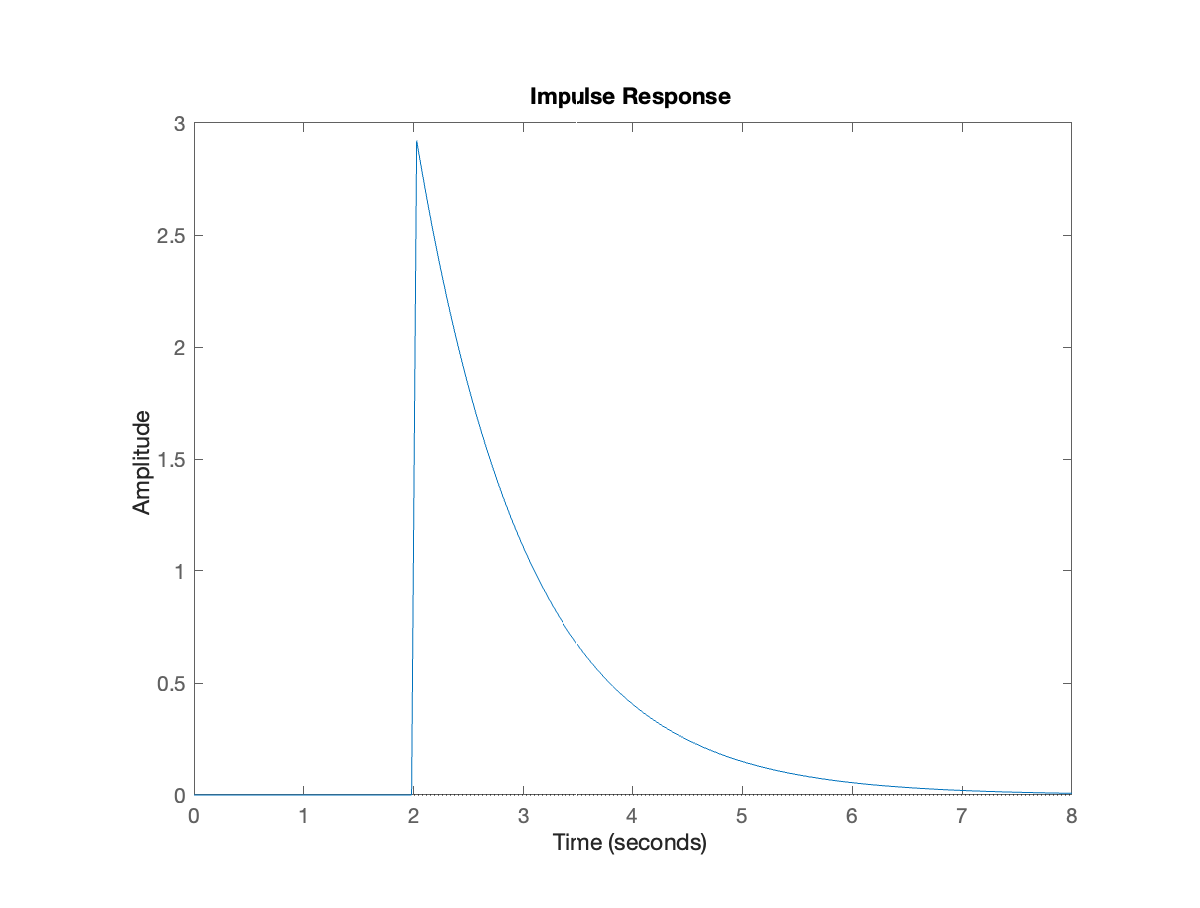
\includegraphics[width=0.8\textwidth]{Bilder/ImpulsAntwortPT1Tt.eps}
    \caption{Impulsantwort}
 \end{figure}

\subsection{Übergangsfunktion (Sprungantwort)}

Die Spungantwort wird auch als Übergangsfunktion $h(t)$ bezeichnet.
Sie ist die Antwort des Systems auf den Einheitssprung $\sigma (t)$.
Ein Beipsiel ist die Heaviside-Funktion, die wie folgt definiert ist:

\[
1 (t) = \begin{cases} 
    0 & \text{für t < 0} \\ 
    \frac{1}{2} & \text{für t = 0} \\
    1 & \text{für t > 0} \end{cases}  
\]

In Matlab lässt sich das mit dem Befehl \texttt{step(sys)} simulieren, wodurch man die numerische Lösung erhält, wie in folgender Abbildung zu sehen.

\begin{figure}[H]
    \label{fig:sprung}
    \centering
    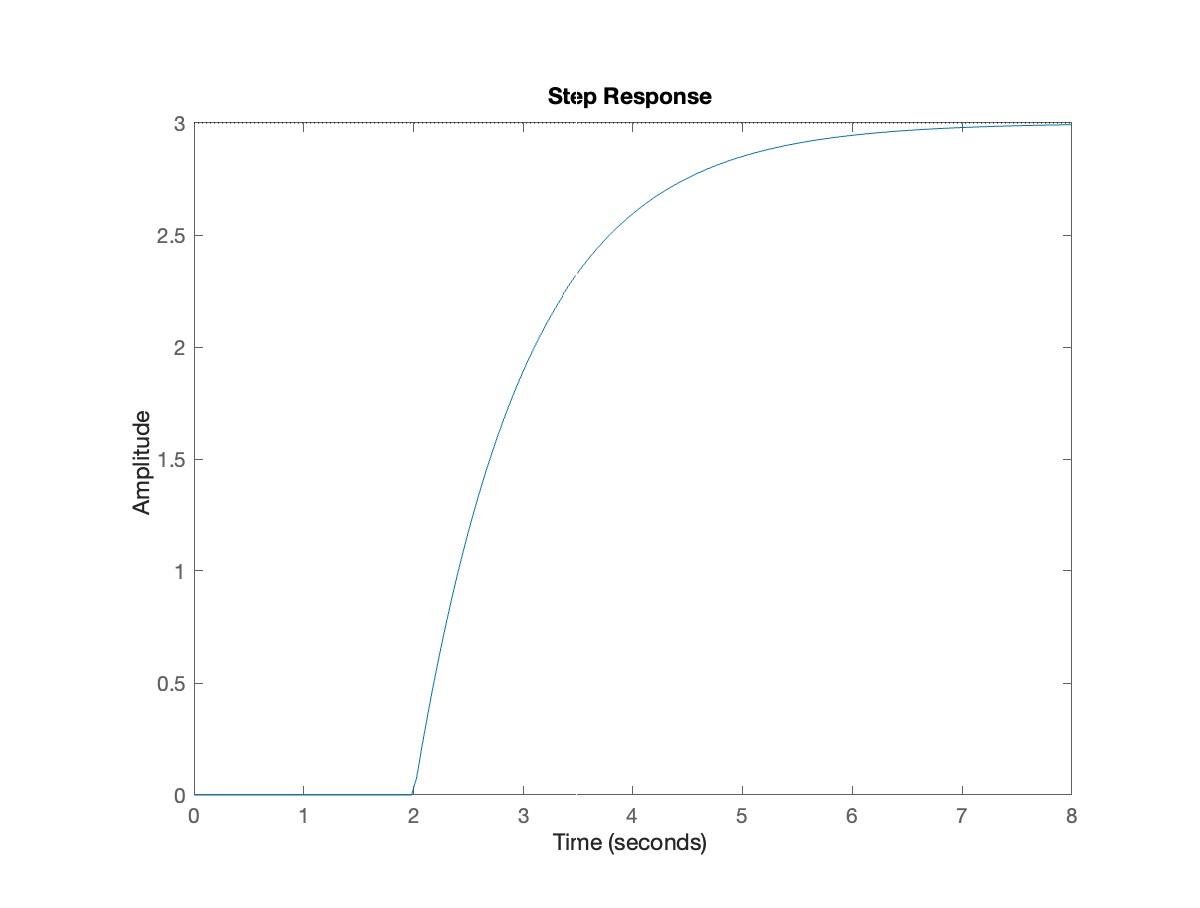
\includegraphics[width=0.8\textwidth]{Bilder/SprungantwortPT1Tt.eps}
    \caption{Sprungantwort}
 \end{figure}

Die Übergangsfunktionfunktion $h(t)$ lässt sich aber auch analytisch berechnen und man erhält die explizite Lösung. Hierbei hilft einem der Befehl \texttt{ilaplace()}, der die Laplace-Transformierte zurückliefert:

\begin{verbatim}
    H(s) = G(s)/s
    syms h(t)
    h(t) = ilaplace(H(s))
\end{verbatim} 

Matlab Ausgabe: \texttt{h(t) = -heaviside(t - 2)*(exp(2 - t) - 1)}\\
Mathematische Notation: 
\begin{align*}
    h(t) &= -1(t-2)\cdot(e^{(2-1)}-1)
\end{align*} wobei $1(t)$ für die Heavyside-Funktion steht.


\subsection{Frequenzgang}
Zum Frequenzgang $G(j \omega)$ gelangt man, indem man in $G(s)$ die Variable $s$ durch $j \omega$ ersetzt.\\
Das $\omega$ steht für die Frequenz in $\frac{rad}{s}$ (Erinnerung: $\omega = 2\pi f$). Das $j$ steht für die imaginäre Einheit, da $i$ in der Systemtheorie für den Strom steht und somit durch $j$ ersetzt wird.

Das bedeutet, dass $G(j \omega)$ für jede Frequzenz $\omega$ eine komplexe Zahl $j$ mit Real- und Imaginärteil oder einen Betrag mit Phase darstellt.
Systemtheoretisch entspricht der Frequenzgang $G(j\omega)$ einem Schnitt der komplexen Funktion von $G(s)$ entlang der imaginären Achse: $G(s)|_{s = j * \omega}$

\subsubsection{Nyquist-Plot (Ortskurve)}
Im Nyquist-Plot wird der über $\omega$ parametrisierte Frequenzgang als Kurve in der komplexen Ebene mit Real- und Imaginärteil dargestellt.

Mit dem Matlab-Befehl \texttt{nyquist(sys)} wird ein Plot der Kurve des Frequenzgangs $G(\omega j)$ ausgegeben. 
Matlab zeigt die Kurve des Frequenzgangs $G(j\omega)$ immer für $\omega$ zwischen $- \infty$ und $+ \infty$ an:

\begin{figure}[H]
    \label{fig:nyquist}
    \centering
    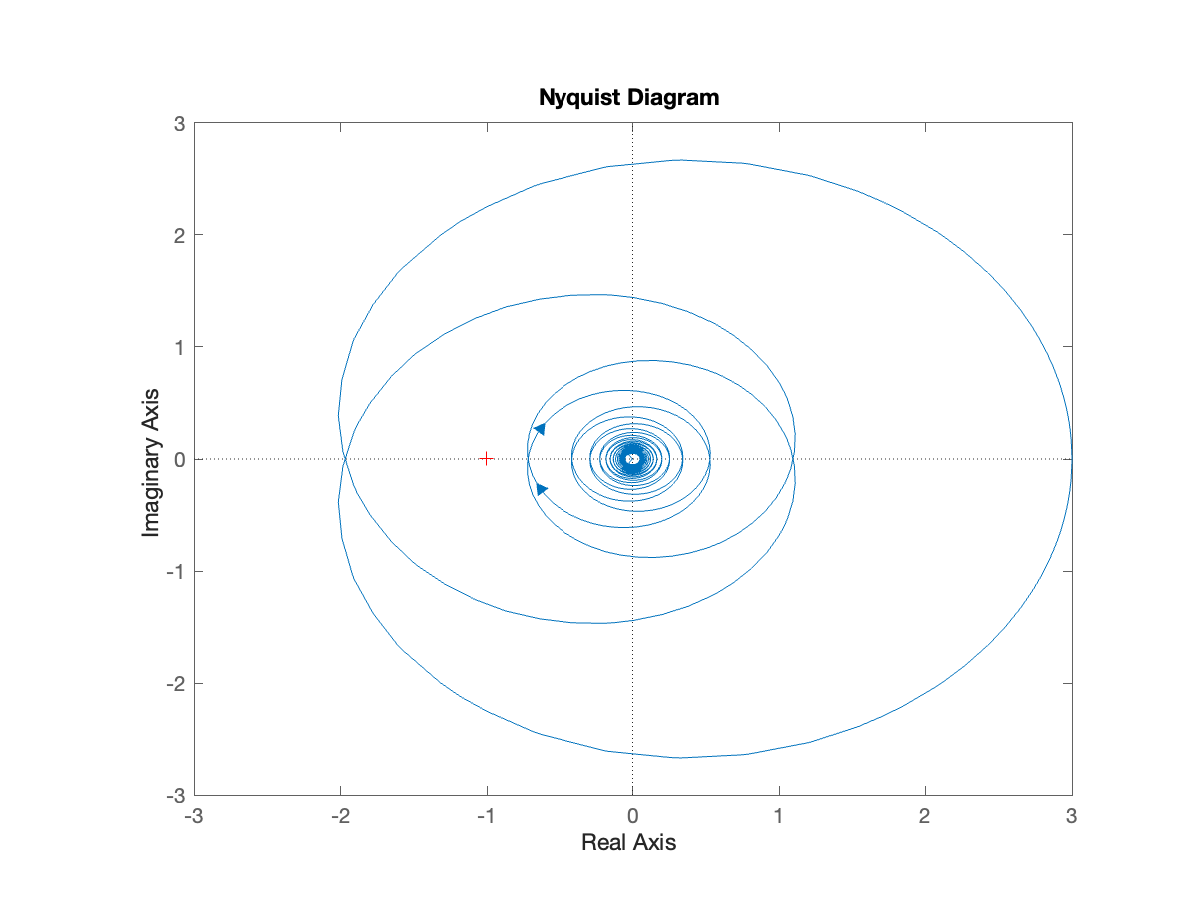
\includegraphics[width=0.8\textwidth]{Bilder/NyquistPT1Tt.eps}
    \caption{Nyquist-Plot}
 \end{figure}

 Dabei ist es möglich, mit dem Cursor entlang der Kurve zu fahren, um sich den Real- und Imaginärteil zu dem jeweiligen Punkt anzeigen zu lassen:
 \begin{figure}[H]
    \label{fig:nyquistCursor}
    \centering
    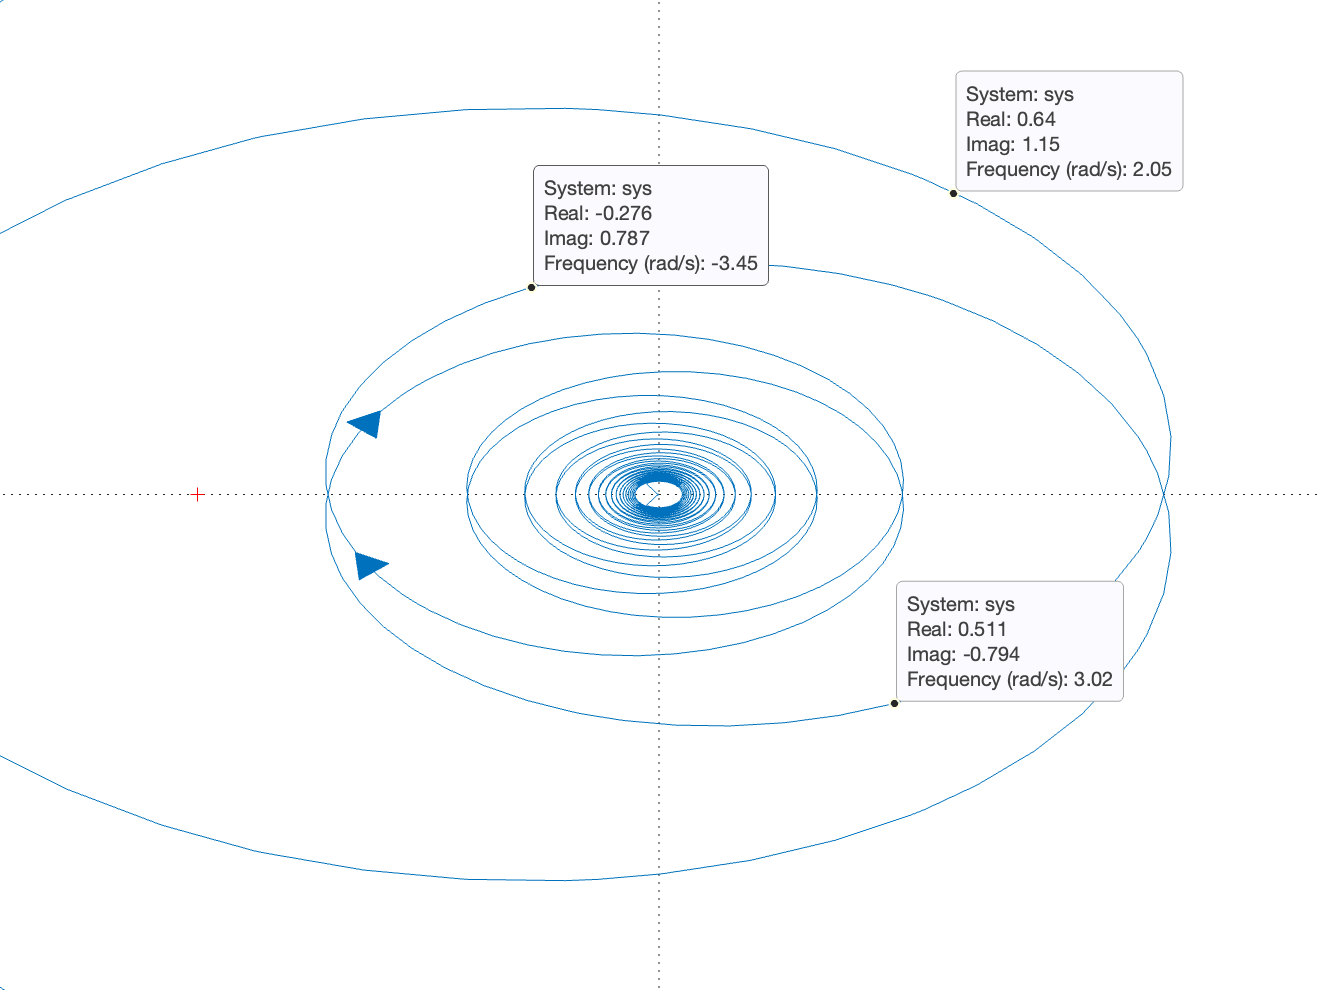
\includegraphics[width=0.6\textwidth]{Bilder/NyquistCursorPT1Tt.png}
    \caption{Screenshot: Informationen im Nyquist-Plot}
 \end{figure}

 
\subsubsection{Bode-Diagramm}
Im Bode-Diagramm sind der Betrag des Frequenzgangs über $\omega$ in Dezibel(dB) und die Phase des Frequenzgangs über $\omega$ in Grad($^\circ$) dargestellt.\\
Streng genommen wird im oberen Diagramm der Abbildung 6 die Amplitudenverstärkung dargestellt, die ein Sinus-Signal an der Frequenz $\omega$ stationär erfährt (wenn die Eigenvorgänge abgeklungen sind und sich das System eingeschwungen hat), während im unteren Diagramm die Phasenverschiebung zu sehen ist.  

Der dazugehörige Matlab-Befehl ist \texttt{bode(sys)}, wobei dieser Befehl intern eine doppelt logarithmische Darstellung verwendet. Die Diagramm-Achse, auf der $\omega$ aufgetragen ist, ist dabei logarithmisch skaliert, während der Betrag in Dezibel (dB) angegeben wird,  damit die Kurven schön aussehen.

\begin{figure}[H]
    \label{fig:bodePlot}
    \label{fig:lassmich}
    \centering
    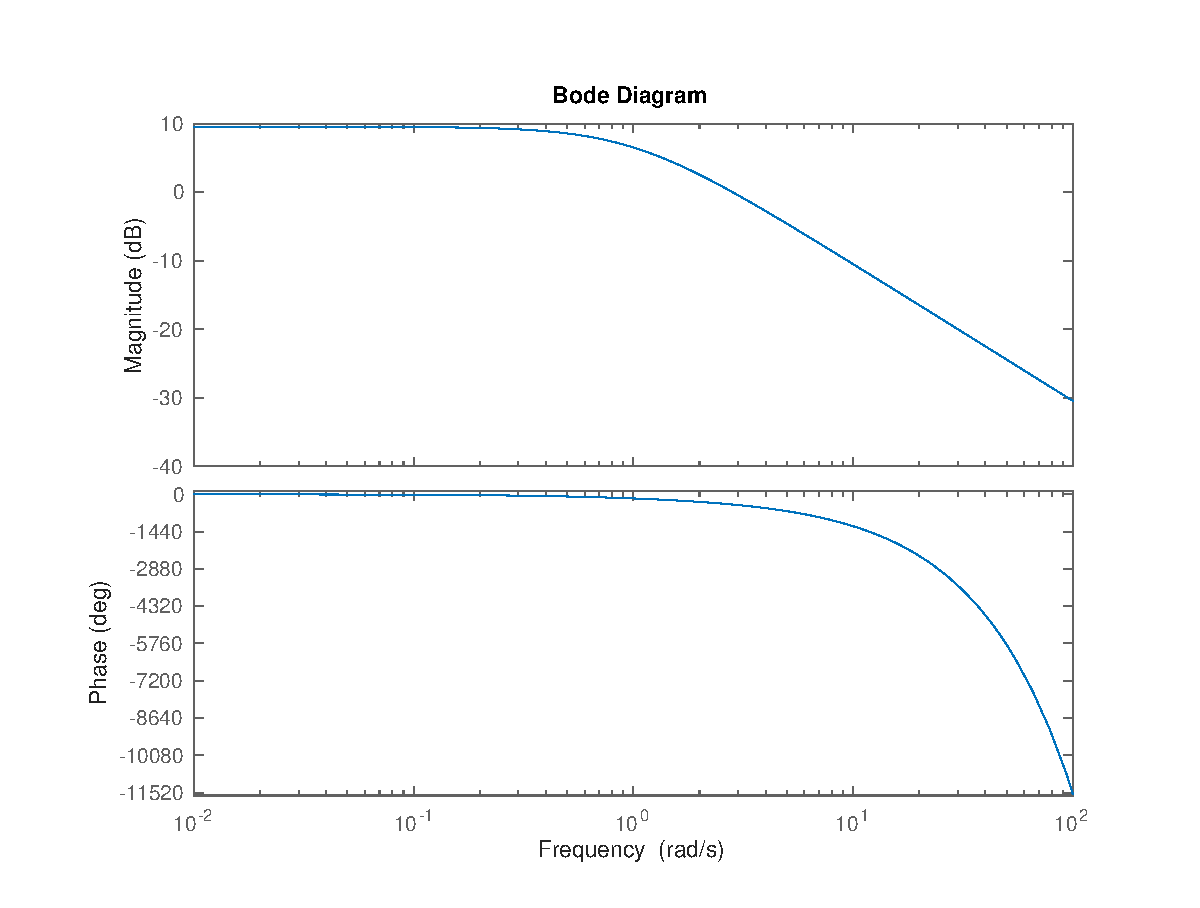
\includegraphics[width=0.8\textwidth]{Bilder/BodePT1Tt.eps}
    \caption{Bode-Plot}
 \end{figure}

\subsubsection{Simulink-Simulation}
Mithilfe von Simulink lässt sich die Übergangsfunktion simulieren. Die Schaltung zeigt den Aufbau mit einem Sinus-Signal als Eingang.
SImulationsscheme
Für 2 Frequenzen ausführen, Amplitudenverstärkung und Phasenverstärkung ablesen
ERgebnis vergleichen mit Bode-Diagramm
Ergebnis vergleichen mit Handrechnungen  -> Muss das gleiche herauskommen

Danach gleiche Schaltung in Integratorform
Bei diesem Bild kann man anderes Eingangssignal wählen und bei Integratoren die Anfangswerte angegebenFormel hinschreiben

\subsection{Statische Kennlinie}

Da es sich bei unserem System um ein System mit proportionalen Übertragungsverhalten handelt, entspricht die statische Verstärkung $K = G(0)$ bzw. $K = \lim_{t\to \infty} h(t)$. 
Somit ergibt sich bei unserem System eine Verstärkung von 1, weshalb die statische Kennlinie nur eine konstante Funktion ist. 

Mithilfe des Matlab-Befehls \texttt{fplot(1)} lässt sich das graphisch darstellen. Der Nachteil der statischen Kennlinie ist, dass sie im Gegensatz zum Pol-Nullstellen-Plot keine Dynamik-Informationen enthält.


\begin{figure}[H]
    \label{fig:staticCurve}
    \centering
    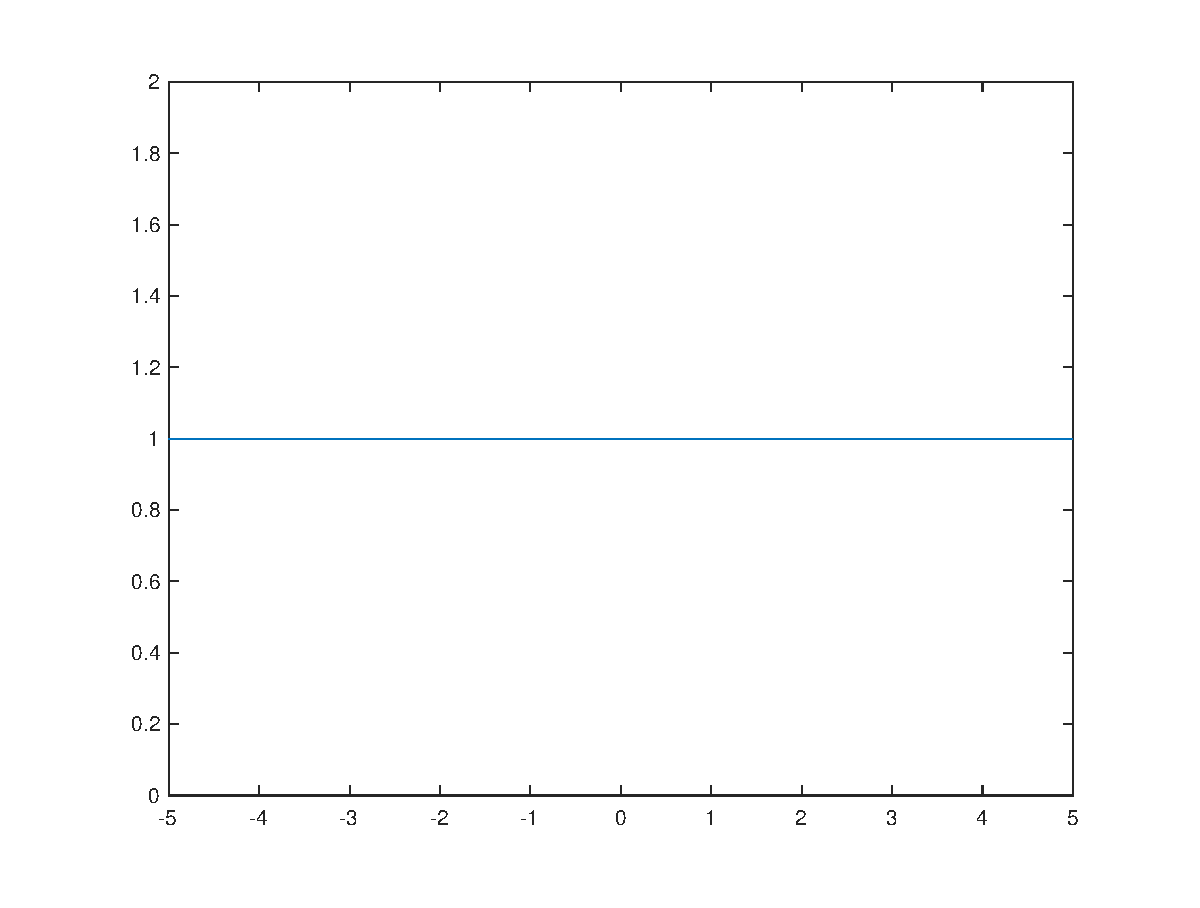
\includegraphics[width=0.8\textwidth]{Bilder/StaticCurvePT1Tt.eps}
    \caption{Statische Kennlinie}
 \end{figure}

\subsection{Pol-Nulstellen-Plot}
Abbildung 9 zeigt den Pol-Nulstellen-Plot zu unserem System. Der passende Matlab-Befehl hierfür lautet \texttt{pzplot(sys)}. Matlab markiert mit \textbf{o} die Nullstellen und mit \textbf{x} die Polstellen des Systems. In unserem Fall hat das System aber keine Nulstellen, da der Zählergrad 0 ist, weshalb in der Abbildung kein \textbf{o} zu sehen ist. Da der Nenner unseres Systems aber den Grad 1 mit $1 + s$ ist, hat unserer System eine reale Polstelle bei s = -1, was in der Abbildung mit den \textbf{x} gekennzeichnet ist. Aufgrund dieses negativen Realteils handelt es sich also um eine stabile Polstelle.
Der Nachteil des Pol-Nullstellen-Plots ist, dass er im Gegensatz zur statischen kennlinie keine Statik-Informationen enthält.

\begin{figure}[H]
    \centering
    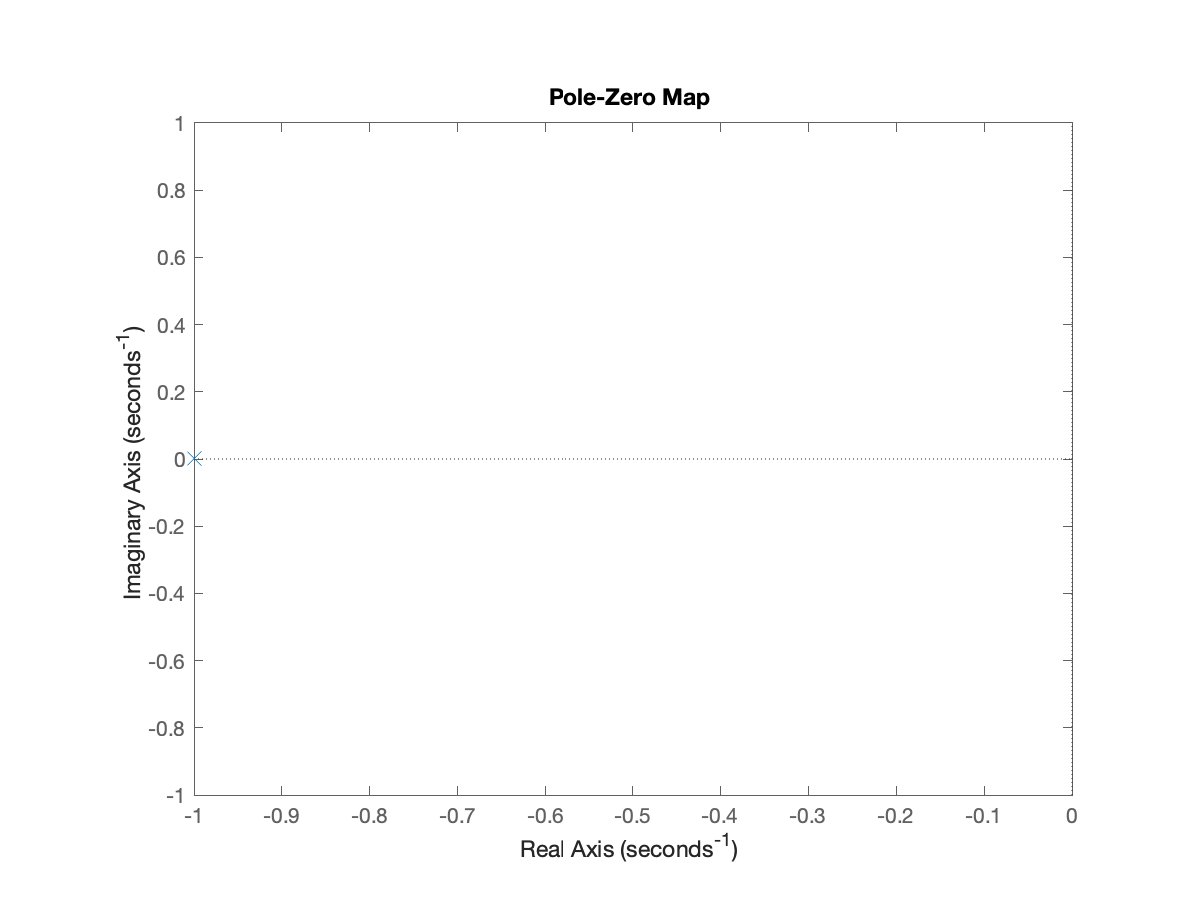
\includegraphics[width=0.8\textwidth]{Bilder/PoleZeroPT1Tt.eps}
    \caption{Pol-Nulstellen-Plot}
 \end{figure}
 %Warum auch immer muss hier das Label nach die Figure und nicht da rein, sonst haben wir ein Problem

